\documentclass[
11pt, % The default document font size, options: 10pt, 11pt, 12pt
%codirector, % Uncomment to add a codirector to the title page
]{charter} 


% El títulos de la memoria, se usa en la carátula y se puede usar el cualquier lugar del documento con el comando \ttitle
\titulo{Asignación de características musicales para ambientación comercial} 

% Nombre del posgrado, se usa en la carátula y se puede usar el cualquier lugar del documento con el comando \degreename
%\posgrado{Carrera de Especialización en Sistemas Embebidos} 
%\posgrado{Carrera de Especialización en Internet de las Cosas} 
\posgrado{Carrera de Especialización en Inteligencia Artificial}
%\posgrado{Maestría en Sistemas Embebidos} 
%\posgrado{Maestría en Internet de las cosas}

% Tu nombre, se puede usar el cualquier lugar del documento con el comando \authorname
% IMPORTANTE: no omitir titulaciones ni tildación en los nombres, también se recomienda escribir los nombres completos (tal cual los tienen en su documento)
\autor{Ing. Carlos Alberto Rivas Araque}

% El nombre del director y co-director, se puede usar el cualquier lugar del documento con el comando \supname y \cosupname y \pertesupname y \pertecosupname
\director{Esp. Ing. Martín Moreyra}
\pertenenciaDirector{GatekeeperX} 
\codirector{} % para que aparezca en la portada se debe descomentar la opción codirector en los parámetros de documentclass
\pertenenciaCoDirector{FIUBA}

% Nombre del cliente, quien va a aprobar los resultados del proyecto, se puede usar con el comando \clientename y \empclientename
\cliente{Carolina Arbelaez}
\empresaCliente{Plusyc Live SAS}
 
\fechaINICIO{26 de agosto de 2025}		%Fecha de inicio de la cursada de GdP \fechaInicioName
\fechaFINALPlan{14 de octubre de 2025} 	%Fecha de final de cursada de GdP
\fechaFINALTrabajo{junio de 2026}	%Fecha de defensa pública del trabajo final


\begin{document}

\maketitle
\thispagestyle{empty}
\pagebreak


\thispagestyle{empty}
{\setlength{\parskip}{0pt}
\tableofcontents{}
}
\pagebreak


\section*{Registros de cambios}
\label{sec:registro}


\begin{table}[ht]
\label{tab:registro}
\centering
\begin{tabularx}{\linewidth}{@{}|c|X|c|@{}}
\hline
\rowcolor[HTML]{C0C0C0} 
Revisión & \multicolumn{1}{c|}{\cellcolor[HTML]{C0C0C0}Detalles de los cambios realizados} & Fecha      \\ \hline
0      & Creación del documento                                 &\fechaInicioName \\ \hline
1      & Se completa hasta el punto 5 inclusive                & {9} de {septiembre} de 2025 \\ \hline
%2      & Se completa hasta el punto 9 inclusive
%		  Se puede agregar algo más \newline
%		  En distintas líneas \newline
%		  Así                                                    & {día} de {mes} de 202X \\ \hline
%3      & Se completa hasta el punto 12 inclusive                & {día} de {mes} de 202X \\ \hline
%4      & Se completa el plan	                                 & {día} de {mes} de 202X \\ \hline

% Si hay más correcciones pasada la versión 4 también se deben especificar acá

\end{tabularx}
\end{table}

\pagebreak



\section*{Acta de constitución del proyecto}
\label{sec:acta}

\begin{flushright}
Buenos Aires, \fechaInicioName
\end{flushright}

\vspace{2cm}

Por medio de la presente se acuerda con el \authorname\hspace{1px} que su Trabajo Final de la \degreename\hspace{1px} se titulará ``\ttitle'' y consistirá en {la implementación de un sistema de generación de características musicales a partir de canciones en el contexto de una aplicación de ambientación musical}. El trabajo tendrá un presupuesto preliminar estimado de {600} horas y un costo estimado de {18750} dólares estadounidenses, con fecha de inicio el \fechaInicioName\hspace{1px} y fecha de presentación pública en \fechaFinalName.

Se adjunta a esta acta la planificación inicial.

\vfill

% Esta parte se construye sola con la información que hayan cargado en el preámbulo del documento y no debe modificarla
\begin{table}[ht]
\centering
\begin{tabular}{ccc}
\begin{tabular}[c]{@{}c@{}}Dr. Ing. Ariel Lutenberg \\ Director posgrado FIUBA\end{tabular} & \hspace{2cm} & \begin{tabular}[c]{@{}c@{}}\clientename \\ \empclientename \end{tabular} \vspace{2.5cm} \\ 
\multicolumn{3}{c}{\begin{tabular}[c]{@{}c@{}} \supname \\ Director del Trabajo Final\end{tabular}} \vspace{2.5cm} \\
\end{tabular}
\end{table}




\section{1. Descripción técnica-conceptual del proyecto a realizar}
\label{sec:descripcion}

%\begin{consigna}{red} % ELIMINAR \begin{consigna}{red} y \end{consigna}{red} en las secciones que vayan completando para cada entrega parcial.
%El objetivo es que el lector, en una o dos páginas, exponga de qué se trata el proyecto y cuáles son sus desafíos, cuál es la motivación para realizarlo y su importancia.

%Se debe introducir el contexto del proyecto, el estado del arte en la temática, describir la propuesta de valor, cuál es el problema que atiende y cuál es la solución que se propone. Se debe dar una descripción funcional de la solución que incluya un diagrama en bloques.

%Puede ser útil incluir en esta sección la respuesta a alguna de estas preguntas:

%\begin{itemize}
%	\item ¿Cuál es el contexto del proyecto, es un emprendimiento personal, un proyecto para una empresa, es parte del programa de vinculación con empresas del posgrado?
%	\item ¿Existen o aplican condiciones especiales al proyecto, financiamiento de algún programa público o privado, acuerdos de confidencialidad, acuerdos sobre la propiedad intelectual de los entregables u otros?
%	\item ¿Cómo se compara la solución propuesta con el estado del arte en el campo de aplicación? ¿En qué aspectos destaca?
%	\item ¿Ayuda a la explicación si se incluye un lienzo Canvas del Modelo de Negocio?
%	\item ¿En qué estado del ciclo de vida está la solución que se propone?
%	\item ¿Cuáles son las características del cliente (el adoptante de los entregables del proyecto) qué valora, qué necesita?
%	\item ¿Por dónde pasa la innovación?
%\end{itemize}

El proyecto se hace para la empresa Plusyc Live SAS, dedicada a la creación de experiencias musicales personalizadas para locales comerciales a través de una aplicación móvil. La aplicación utiliza un \textit{pool} de canciones propio, y un \textit{backend} que crea listas de reproducción. Las listas se generan gracias a características musicales, tales como el género, ánimo, energía y tempo de cada canción. Actualmente, la asignación de características musicales depende del acceso a interfaces de programación de aplicaciones (API) de terceros, lo que genera restricciones de disponibilidad y costos. Esto afecta la escalabilidad y autonomía del sistema, y en consecuencia, la calidad de la experiencia ofrecida a los clientes.

Se propone el desarrollo de un sistema de inteligencia artificial (IA) que reciba como entrada canciones y genere como salida sus características musicales. Se entrenarán y evaluarán modelos de aprendizaje supervisado, a partir de técnicas y representaciones numéricas del sonido, fuentes de datos privadas de la empresa, y datos públicos disponibles. Y se podrán inferir las características de nuevas canciones sin depender de proveedores externos.

En el ámbito de la inteligencia artificial aplicada a la música, existen herramientas que permiten extraer información musical a bajo nivel, y herramientas en línea que permiten extraer algunas características específicas. Sin embargo, no se cuenta con una solución que provea resultados completos y resuelva el problema de la disponibilidad.

La propuesta de valor radica en otorgar a Plusyc Live SAS una solución completa, integrada y altamente disponible, en pro de la escalabilidad y la independencia tecnológica. Los comercios tendrán una renovación en la experiencia de sus consumidores. El sistema será además reutilizable en otros proyectos de la empresa.

A continuación, en la figura 1, se presenta el diagrama de bloques de alto nivel de la aplicación. A la derecha del diagrama se observa el sistema basado en IA, que es el foco del proyecto. 
%La descripción técnica-conceptual \textbf{debe incluir al menos un diagrama en bloques del sistema} y descripción funcional de la solución propuesta.

%Las figuras se deben mencionar en el texto ANTES de que aparezcan con una frase como la siguiente: ``En la figura \ref{fig:diagBloques} se presenta el diagrama en bloques del sistema. Se observa que...''.  La regla es que las figuras nunca pueden ir antes de ser mencionadas en el texto, porque sino el lector no entiende por qué de pronto aparece una figura.

\begin{figure}[htpb]
\centering 
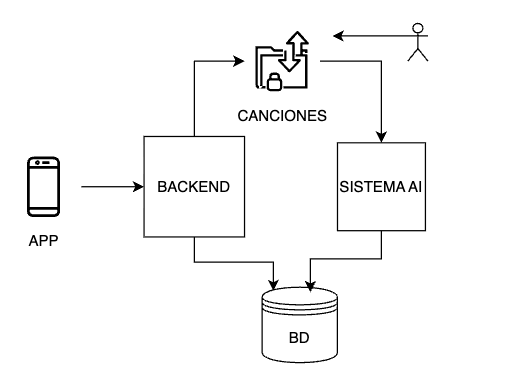
\includegraphics[width=.65\textwidth]{./Figuras/diagBloques.png}
\caption{Diagrama en bloques del sistema.}
\label{fig:diagBloques}
\end{figure}

\vspace{25px}
En la figura se puede observar un actor que provee los archivos de las canciones que son las entradas del sistema IA, donde se procesa cada canción para extraer sus características musicales. Las características son las salidas, y son almacenadas en una base de datos que alimenta el \textit{backend} de la aplicación. Ahora, en la figura 2, se muestra un diagrama de bloques más detallado del sistema IA. 

\begin{figure}[htpb]
\centering 
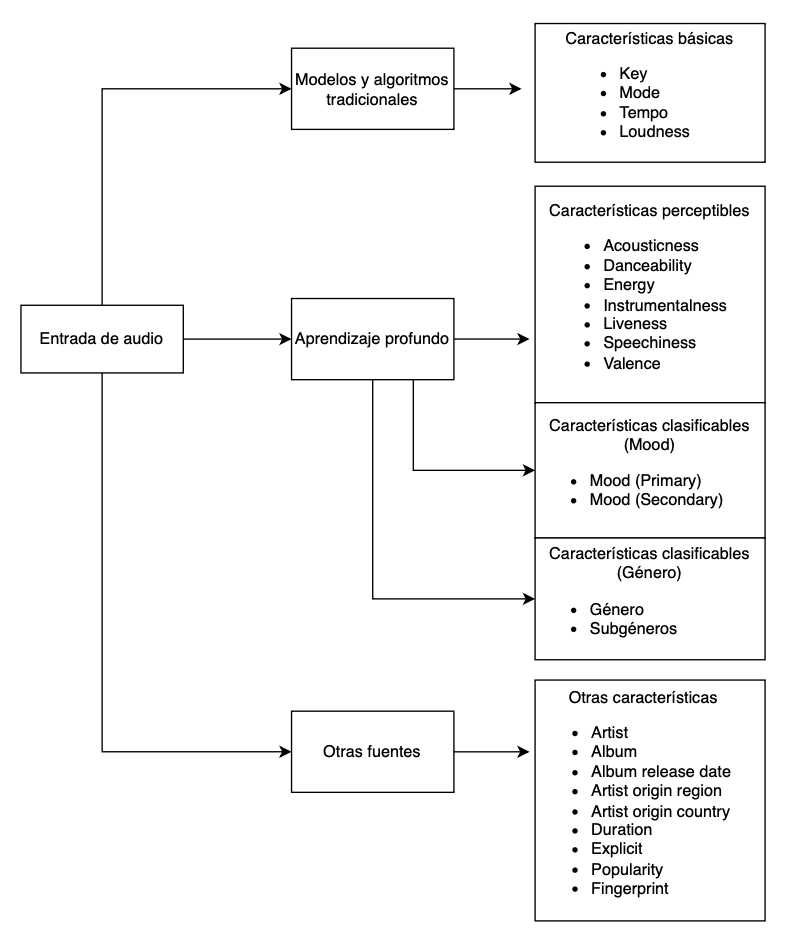
\includegraphics[width=.65\textwidth]{./Figuras/diagBloques2.png}
\caption{Diagrama de bloques del sistema IA.}
\label{fig:diagBloques}
\end{figure}

\vspace{25px}
En la figura se observa que el sistema IA utiliza tres módulos principales: ``Modelos y algoritmos tradicionales'', ``Aprendizaje profundo'' y ``Otras fuentes''. Cada módulo procesa el archivo de audio y se encarga de inferir o consultar un subconjunto específico de características musicales.

%El tamaño del texto en TODAS las figuras debe ser adecuado \textbf{para que NO pase lo que ocurre en la figura \ref{fig:diagBloques}}, donde el lector debe esforzarse para poder leer el texto. 

%Los colores usados en el diagrama deben ser adecuados, tal que ayuden a comprender mejor el diagrama. Se recomienda evitar colores primarios (como rojo, verde o cyan) y usar la gama de colores pastel.

%\end{consigna} % ELIMINAR \begin{consigna}{red} y \end{consigna}{red} en las secciones que vayan completando para cada entrega parcial.

\section{2. Identificación y análisis de los interesados}
\label{sec:interesados}

%\begin{consigna}{red} % ELIMINAR \begin{consigna}{red} y \end{consigna}{red} en las secciones que vayan completando para cada entrega parcial.
%\textbf{Nota importante:} borrar esto y todas las consignas en color rojo antes de entregar este documento). Esto se hace eliminando el par de comandos que forman el bloque consigna, \verb!\begin{consigna}{red}! y \verb!\end{consigna}{red}! del código. 
 
%Es inusual que una misma persona esté en más de un rol, incluso en proyectos chicos. Si se considera que una persona cumple dos o más roles, entonces \textbf{solo dejarla en el rol más importante}. 

%Por ejemplo, si una persona es Cliente pero también colabora u orienta, dejarla solo como Cliente. Si una persona es el Responsable, \textbf{no debe ser colocado también como miembro del equipo}.


%El Director suele ser uno de los orientadores.

%No dejar celdas vacías; si no hay nada que poner en una celda colocar un signo ``-''.

%No dejar filas vacías; si no hay nada que poner en una fila entonces eliminarla.

%Es deseable listar a continuación las principales características de cada interesado.
 
%Por ejemplo:

\begin{itemize}
	\item Cliente: \clientename, es la encargada de aprobar los entregables.
  \item Impulsor: el Ing. Andrés Saldarriaga, es el responsable de brindar acceso a los datos del cliente, y las herramientas tecnológicas necesarias en producción, como credenciales, y proveedores de infraestructura en la nube.
  \item Responsable: \authorname, es quien llevará a cabo el desarrollo del proyecto.
	\item Orientador: \supname, es experto en solución de problemas de inteligencia artificial y va a ser consultor y ayuda para resolver problemas puntuales en caso de \textit{blockers} técnicos.
  \item Usuario final: el usuario final son los clientes de Plusyc Live SAS, que utilizan la aplicación para ambientar su comercio con listas personalizadas.
\end{itemize}

\begin{table}[ht]
%\caption{Identificación de los interesados}
%\label{tab:interesados}
\begin{tabularx}{\linewidth}{@{}|l|X|X|l|@{}}
\hline
\rowcolor[HTML]{C0C0C0} 
Rol           & Nombre y Apellido & Organización 	& Puesto 	\\ \hline
%Auspiciante   &                   &              	&        	\\ \hlineRol           & Nombre y Apellido & Organización 	& Puesto 	\\ \hline
Cliente       & \clientename      &\empclientename	& C.E.O.	\\ \hline
Impulsor      & Ing. Andrés Saldarriaga  &\empclientename   & C.T.O.  \\ \hline
Responsable   & \authorname       & FIUBA        	& Alumno 	\\ \hline
%Colaboradores &                   &              	&        	\\ \hline
Orientador    & \supname	      & \pertesupname 	& Director del Trabajo Final \\ \hline
%Equipo        & miembro1 \newline 
%				miembro2          &              	&        	\\ \hline
%Opositores    &                   &              	&        	\\ \hline
Usuario final & -                   & -              	& Locales comerciales        	\\ \hline
\end{tabularx}
\end{table}

%\end{consigna} % ELIMINAR \begin{consigna}{red} y \end{consigna}{red} en las secciones que vayan completando para cada entrega parcial.

\section{3. Propósito del proyecto}
\label{sec:proposito}

%\begin{consigna}{red} % ELIMINAR \begin{consigna}{red} y \end{consigna}{red} en las secciones que vayan completando para cada entrega parcial.

%¿Por qué se hace el proyecto? ¿Qué se quiere lograr? 

%Se recomienda que sea solo un párrafo que continúe con la idea de la frase ``el propósito de este proyecto es...'' (omitir la frase, ya que está en el título de la sección).
%\end{consigna}

Desarrollar un sistema de inteligencia artificial capaz de caracterizar automáticamente canciones a partir de su archivo de audio, con el fin de reducir la dependencia de servicios externos y garantizar la escalabilidad, autonomía y confiabilidad de la aplicación de Plusyc Live SAS. Con ello, se busca fortalecer la experiencia musical personalizada que la empresa ofrece a los comercios y abrir la posibilidad de aplicar esta tecnología en otros contextos dentro del sector musical.

\section{4. Alcance del proyecto}
\label{sec:alcance}

%\begin{consigna}{red}
%¿Qué se incluye y que no se incluye en este proyecto?

%Se refiere al trabajo que se va a hacer para entregar el producto o resultado especificado. 

%Explicitar todo lo quede comprendido dentro del alcance del proyecto. Por ejemplo:

Se definen los siguientes subconjuntos de características musicales:
\begin{itemize}
  \item Básicas: \textit{\{Key, Mode, Tempo, Loudness\}}.
  \item Perceptibles: \textit{\{Danceability, Energy, Speechiness, Acousticness, Instrumentalness, Liveness, Valence\}}.
  \item Clasificables por ánimo (\textit{Mood}): \textit{\{Primary Mood, Secondary Mood\}}.
  \item Clasificables por género: \textit{\{Genre, Subgenres\}}.
  \item Otras (Aquellas que no requiren de IA para su asignación): \textit{\{Artist, Album, Album release date, Artist origin region, Artist origin country, Duration, Explicit, Popularity, Fingerprint\}}.
\end{itemize}

El proyecto incluye la asignación de las características básicas, perceptibles y las clasificables por ánimo y género. Para lograr esto es necesario:

\begin{itemize}
  \item Revisión del estado del arte sobre \textit{datasets} musicales disponibles para modelos de aprendizaje supervisado (algoritmos tradicionales) y aprendizaje profundo.
  \item Evaluación de los datos del cliente para verificar volumen, calidad de asignaciones y posibilidad de conformar un \textit{dataset} propio.
  \item Análisis de audio, representaciones numéricas de señales de audio para depurar los \textit{datasets}.
  \begin{itemize}
    \item Extracción de representaciones tradicionales para los modelos supervisados.
		\item Generación de representaciones intermedias para aprendizaje profundo.
	\end{itemize}
  \item Depuración de los \textit{datasets} para los modelos de aprendizaje supervisado tradicionales.
	\item Elección de modelos de aprendizaje supervisado y algoritmos tradicionales para la predicción de las características básicas.
  \item Evaluación de los \textit{datasets} para modelos de aprendizaje profundo.
  \item Selección de modelos de aprendizaje profundo y modelos preentrenados para la inferencia de características perceptibles, y clasificables por ánimo y género.
  \item Implementación de los modelos seleccionados.
  \item Construcción de un  \textit{pipeline} para la asignación de características mediante el uso de los modelos seleccionados como los mejores.
  \item Almacenamiento de las características de salida en la base de datos.
\end{itemize}

%Explicitar además todo lo que no quede incluido (``El presente proyecto no incluye...'')

%\end{consigna} % ELIMINAR \begin{consigna}{red} y \end{consigna}{red} en las secciones que vayan completando para cada entrega parcial.

El presente proyecto no incluye:
\begin{itemize}
  \item Asignación del subconjunto de otras características que no requieren de IA para su asignación.
  \item Desarrollo de una interfaz para la recepción de un nuevo archivo de audio.
  \item Desarrollo de interfaces gráficas de usuario.
  \item Puesta en producción del sistema en un entorno del cliente.
  \item Mantenimiento y monitoreo a largo plazo.
\end{itemize}

\section{5. Supuestos del proyecto}
\label{sec:supuestos}

%\begin{consigna}{red} % ELIMINAR \begin{consigna}{red} y \end{consigna}{red} en las secciones que vayan completando para cada entrega parcial.
Para el desarrollo del presente proyecto se supone:

\begin{itemize}
	\item Disponibilidad de recursos de \textit{hardware}: se dispondría de acceso a instancias de procesamiento locales, y en la nube con los suficientes recursos para las fases de entrenamiento y validación de los modelos.
	\item Disponibilidad de datos para el entrenamiento del modelo de procesamiento de audio: se tendría acceso a un conjunto diverso de datos de audio que cubrirán una amplia gama de géneros y estilos.
	\item Factibilidad técnica: se asume que las tecnologías actuales de procesamiento de audio son lo suficientemente avanzadas para implementar el proyecto. Y en particular.
  \begin{itemize}  
    \item Las características básicas se pueden generar usando modelos de aprendizaje de máquina y algoritmos tradicionales.
    \item Las perceptibles y las clasificables por ánimo y género se pueden predecir usando un modelos de aprendizaje profundo de múltiples salidas.
  \end{itemize}    
  \item Tiempo: se estima que las 600 horas asignadas para el desarrollo del proyecto serán suficientes para completar todas las etapas, incluyendo la planeación, análisis y diseño, desarrollo, pruebas y potenciales correcciones del sistema.
  \item Asistencia de los interesados: se contaría con la ayuda del cliente ante \textit{blockers} técnicos, y dudas sobre los requisitos del sistema.
\end{itemize}

%Por ejemplo, se podrían incluir supuestos respecto a disponibilidad de tiempo y recursos humanos y materiales, sobre la factibilidad técnica de distintos aspectos del proyecto, sobre otras cuestiones que sean necesarias para el éxito del proyecto como condiciones macroeconómicas o reglamentarias.

%\end{consigna} % ELIMINAR \begin{consigna}{red} y \end{consigna}{red} en las secciones que vayan completando para cada entrega parcial.

\section{6. Product Backlog}
\label{sec:backlog}

%El Product Backlog debe organizarse en cuatro \textbf{\textit{\'{e}picas}} fundamentales del proyecto. Cada \'{e}pica debe contener al menos dos historias de usuario que describan funcionalidades clave.

%El Product Backlog debe permitir interpretar cómo será el proyecto y su funcionalidad. Se deben indicar claramente las prioridades entre las historias de usuario y si hay alguna opcional.

%Las historias de usuario deben ser breves, claras y medibles, expresando el rol, la necesidad y el propósito de cada funcionalidad. También deben tener una prioridad definida para facilitar la planificación de los sprints.

%Cada historia de usuario debe incluir una ponderación en \textit{Story Points}, un número entero que representa el tama\~no relativo de la historia. El criterio para calcular los Story Points debe indicarse explícitamente.

%Las historias deben seguir el formato: ``\textit{Como [rol], quiero [tal cosa] para [tal otra cosa]}''.

%Las \'{e}picas deben estructurarse de la siguiente forma:


Se definen los siguientes roles:

\begin{itemize}
	\item Usuario: la persona del lado del cliente con conocimientos en características musicales, para verificar que las salidas son correctas.
	\item Desarrollador de software con conocimiento en inteligencia artificial: la persona ocupando este rol deberá tener conocimiento suficiente en procesamiento de audio, y entrenamiento de modelos de inteligencia artificial, para la generación de características musicales.
	\item Cliente: es el encargado de verificar que el proyecto cumple con las especificaciones, y dar la aprobación final del sistema.
\end{itemize}

Épicas, historias de usuario (HU) y \textit{spikes}:

Se llevarán a cabo sprints de 2 semanas, y cada sprint tendrá una dedicación de aproximadamente 40 horas. Para la estimación del total de Story Points (SP) se usa la serie de Fibonacci. Se suman las ponderaciones de dificultad, complejidad e incertidumbre, y se aproxima al inmediato superior de la serie.

\begin{itemize}
  \item \textbf{Selección de \textit{datasets} y técnicas de representación de audio}
    \begin{itemize}
      \item \textbf{\textit{Spike} 1:}
      como desarrollador de IA, quiero encontrar \textit{datasets} musicales públicos, y técnicas de representación de audio para ser usados en algoritmos y modelos tradicionales.
      
      Prioridad máxima, 3 SP (complejidad: 1, dificultad: 1, incertidumbre: 1)
      \item \textbf{\textit{Spike} 2:}
      como desarrollador de IA, quiero determinar cuales \textit{datasets} musicales públicos, y técnicas de representación de audio, se usarán para aprendizaje profundo.      
      
      Prioridad máxima, 2 SP (complejidad: 1, dificultad: 1, incertidumbre: 0)
      \item \textbf{\textit{Spike} 3:}
      como desarrollador de IA, quiero evaluar los datos del cliente, en términos de volumen y calidad, para determinar si es posible conformar un \textit{dataset} propio.
      
      Prioridad alta, 2 SP (complejidad: 1, dificultad: 1, incertidumbre: 1)
      \vspace{2cm}
    \end{itemize}
  \vspace{2cm}
  \item \textbf{Desarrollo de algoritmos y modelos tradicionales para características básicas}
    \begin{itemize}
      \item \textbf{HU 1:}
      como desarrollador de IA, quiero realizar un análisis exploratorio de datos (EDA) de las característica básicas, para entender su distribución.
      
      Prioridad alta, 5 SP (complejidad: 2, dificultad: 2, incertidumbre: 1)
      \item \textbf{HU 2:}
      como desarrollador de IA, quiero preparar los datos para que sean aptos para el modelado.
      
      Prioridad alta, 5 SP (complejidad: 2, dificultad: 2, incertidumbre: 1)
      \item \textbf{HU 3:}
      como desarrollador de IA, quiero entrenar modelos tradicionales para predecir cada una de las características básicas.
      
      Prioridad alta, 5 SP (complejidad: 2, dificultad: 2, incertidumbre: 1)
      \item \textbf{HU 4:}
      como desarrollador de IA, quiero evaluar los resultados del modelo con métricas apropiadas, para validar su calidad, y seleccionar el mejor.
      
      Prioridad alta, 5 SP (complejidad: 2, dificultad: 2, incertidumbre: 1)
    \end{itemize}
  \item \textbf{Desarrollo de modelos de aprendizaje profundo para características perceptibles}
    \begin{itemize}
      \item \textbf{HU 5:}
      como desarrollador de IA, quiero realizar un EDA de los datos de las características perceptibles, para entender su distribución y correlaciones.
      
      Prioridad alta, 5 SP (complejidad: 2, dificultad: 2, incertidumbre: 1)
      \item \textbf{HU 6:}
      como desarrollador de IA, quiero preparar los datos de audio para entrenar un modelo.
      
      Prioridad alta, 5 SP (complejidad: 2, dificultad: 2, incertidumbre: 1)
      \item \textbf{HU 7:}
      como desarrollador de IA, quiero entrenar un modelo multi-salida de aprendizaje profundo para predecir las características perceptibles.
      
      Prioridad alta, 5 SP (complejidad: 2, dificultad: 2, incertidumbre: 1)
      \item \textbf{HU 8:}
      como desarrollador de IA, quiero evaluar los resultados del modelo con métricas apropiadas para validar su desempeño.
      
      Prioridad alta, 5 SP (complejidad: 2, dificultad: 2, incertidumbre: 1)
      
    \end{itemize}
  \item \textbf{Desarrollo de modelos de aprendizaje profundo para características clasificables por ánimo}
    \begin{itemize}
      \item \textbf{HU 9:}
      como desarrollador de IA, quiero realizar un EDA de los datos de las características clasificables por ánimo, para analizar su distribución y categorías.
      
      Prioridad alta, 3 SP (complejidad: 1, dificultad: 1, incertidumbre: 1)
      \item \textbf{HU 10:}
      como desarrollador de IA, quiero preparar los datos para el modelado de \textit{moods}.
      
      Prioridad alta, 3 SP (complejidad: 1, dificultad: 1, incertidumbre: 1)
      \item \textbf{HU 11:}
      como desarrollador de IA, quiero entrenar un modelo multi-salida de aprendizaje profundo para predecir \textit{primary} y \textit{secondary mood}.
      
      Prioridad alta, 3 SP (complejidad: 1, dificultad: 1, incertidumbre: 1)
      \item \textbf{HU 12:}
      como desarrollador de IA, quiero evaluar el modelo con métricas de clasificación multi-clase para validar su desempeño.
      
      Prioridad alta, 3 SP (complejidad: 1, dificultad: 1, incertidumbre: 1)
      \vspace{2cm}
    \end{itemize}

  \item \textbf{Desarrollo de modelos de aprendizaje profundo para características clasificables por género}
    \begin{itemize}
      \item \textbf{HU 13:}
      como desarrollador de IA, quiero realizar un EDA de los datos de géneros y subgéneros para entender su distribución y categorías.
      
      Prioridad alta, 3 SP (complejidad: 1, dificultad: 1, incertidumbre: 1)
      \item \textbf{HU 14:}
      como desarrollador de IA, quiero preparar los datos para modelado de género.
      
      Prioridad alta, 3 SP (complejidad: 1, dificultad: 1, incertidumbre: 1)
      \item \textbf{HU 15:}
      como desarrollador de IA, quiero entrenar un modelo multi-salida de aprendizaje profundo para predecir el género y los subgéneros.
      
      Prioridad alta, 3 SP (complejidad: 1, dificultad: 1, incertidumbre: 1)
      \item \textbf{HU 16:}
      como desarrollador de IA, quiero evaluar los resultados del modelo con métricas de clasificación, para validar su desempeño.
      
      Prioridad alta, 3 SP (complejidad: 1, dificultad: 1, incertidumbre: 1)
    \end{itemize}        
  \item \textbf{Implementación del  \textit{pipeline} de procesamiento}
    \begin{itemize}
      \item \textbf{HU 17 - opcional:}
      como cliente, quiero una interfaz para la recepción de un nuevo archivo de audio, para alimentar el \textit{pipeline} que genere las características musicales.
      
      Prioridad baja, 8 SP (complejidad: 3, dificultad: 2, incertidumbre: 1)
      \item \textbf{HU 18:}
      como cliente, quiero un \textit{pipeline} que procese los modelos desarrollados para automatizar la generación de características musicales, y almacenar los resultados en una base de datos.
      
      Prioridad media, 8 SP (complejidad: 3, dificultad: 2, incertidumbre: 1)
      \item \textbf{HU 19 - opcional:}
      como cliente, quiero desplegar el sistema en el \textit{backend}, para automatizar la generación de características musicales del audio en producción.
      
      Prioridad baja, 13 SP (complejidad: 5, dificultad: 3, incertidumbre: 1)
      \item \textbf{HU 20:}
      como usuario, quiero tener acceso de lectura a la base de datos para validar la calidad de las características resultantes.
      
      Prioridad alta, 3 SP (complejidad: 1, dificultad: 1, incertidumbre: 1)      
    \end{itemize}
\end{itemize}

%\textbf{Reglas para definir historias de usuario:}
%\begin{itemize}
%  \item Ser concisas y claras.
%  \item Expresarlas en términos cuantificables y medibles.
%  \item No dejar margen para interpretaciones ambiguas.
%  \item Indicar claramente su prioridad y si son opcionales.
%  \item Considerar regulaciones y normas vigentes.
%\end{itemize}

\section{7. Criterios de aceptación de historias de usuario}
\label{sec:criteriosAceptacion}

%Los criterios de aceptación deben establecerse para cada historia de usuario, asegurando que se cumplan las condiciones necesarias para que la funcionalidad sea validada correctamente.

%Cada historia debe tener criterios medibles, específicos y verificables. Deben permitir validar que se cumple con las necesidades del usuario.

%Se estructuran de forma análoga a las \'{e}picas del backlog:

\begin{itemize}
  \item \textbf{Selección de \textit{datasets} y técnicas de representación de audio}
    \begin{itemize}
      \item \textbf{Spike 1}
      \begin{itemize}
        \item Se genera un documento que incluye los hallazgos de \textit{datasets} públicos, con ventajas y desventajas.
        \item Se listan y detallan las representaciones de audio disponibles.
        \item Se dispone de criterios de uso de los \textit{datasets} y representaciones de audio para el conjunto de características básicas.
      \end{itemize}
      \item \textbf{Spike 2}
      \begin{itemize}
        \item Se extiende el documento anterior con otros \textit{datasets} específicos en el marco del aprendizaje profundo.
        \item Se agregan las representaciones de audio disponibles en este marco.
        \item Se añaden los criterios de uso de de los \textit{datasets} y representaciones de audio para los conjuntos de características perceptibles y de clasificación.
      \end{itemize}      
      \item \textbf{Spike 3}
      \begin{itemize}
        \item Se incluye un resumen del inventario de datos privados del cliente, audios y características.
        \item Se describe la calidad de los datos en términos de la consistencia de las características asignadas.
        \item Se concluye si es viable construir y usar un \textit{dataset} propio.
      \end{itemize}   
    \end{itemize}

  \item \textbf{Desarrollo de algoritmos y modelos tradicionales para características básicas, perceptibles y clasificables por ánimo y género}
    \begin{itemize}
      \item \textbf{HU 1, HU 5, HU 9 y HU 13}
      \begin{itemize}
        \item Se presenta un análisis exploratorio de datos con estadísticas descriptivas.
        \item Se identifican las distribuciones y correlaciones de los datos según gráficos y visualizaciones.
        \item El informe muestra el tratamiento de valores nulos o atípicos.
        \item Se describen las categorías del problema de clasificación: Aplica en HU 9, HU 13, y para \textit{Key} y \textit{Mode} en HU 1.
      \end{itemize}
      \item \textbf{HU 2, HU 6, HU 10 y HU 14}
      \begin{itemize}
        \item Se realiza la normalización o estandarización de datos numéricos según aplique.
        \item Se codifican variables categóricas con técnicas estándar (p. ej., \textit{one-hot encoding}) según aplique.
        \item Se documentan los pasos de limpieza de datos y el tratamiento de valores faltantes.
      \end{itemize}
      \item \textbf{HU 3, HU 7, HU 11 y HU 15}
      \begin{itemize}
        \item En HU 3 se implementa al menos un modelo tradicional de aprendizaje supervisado, como máquinas de vectores de soporte (SVM), árboles aleatorios (RF), o k vecinos cercanos (kNN).
        \item Se ejecutan algoritmos tradicionales (sin IA) para comparar los resultados con los resultados del modelo tradicional. Aplica en el caso de HU 3.
        \item En HU 7, HU 11 y HU 15, se implementa al menos un modelo de red neuronal.
        \item Se documenta el proceso de selección de hiperparámetros en un \textit{Jupyter noteobok}.
      \end{itemize}
      \item \textbf{HU 4, HU 8, HU 12 y HU 16}
      \begin{itemize}
        \item Se aplican métricas de desempeño (p. ej., \textit{accuracy}, \textit{F1}, \textit{RMSE} según el caso).
        \item Se selecciona el mejor modelo o algoritmo por característica en función de estas métricas.
        \item Se entrega reporte comparativo de modelos y algoritmos.
      \end{itemize}
    \end{itemize}

  \item \textbf{Implementación del  \textit{pipeline} de procesamiento}
    \begin{itemize}
      \item \textbf{HU 17 - opcional}
      \begin{itemize}
        \item La interfaz permite subir archivos de audio en formato estándar (.mp3 o .wav).
        \item Cada archivo se agrega a la cola de procesamiento.
        \item El sistema devuelve confirmación de recepción.
        \vspace{2cm}
      \end{itemize}
      \item \textbf{HU 18}
        \begin{itemize}
        \item El \textit{pipeline} procesa automáticamente un archivo nuevo.
        \item Se ejecutan los modelos desarrollados.
        \item Los resultados se almacenan en la base de datos.
        \item El sistema almacena estado y detalle asociado al archivo.
        \end{itemize}
      \item \textbf{HU 19 - opcional}
      \begin{itemize}
        \item El sistema está disponible en un entorno de producción del cliente.
        \item El \textit{backend} permite ejecutar al menos 10 archivos consecutivos sin fallo.
        \item La documentación de despliegue está disponible para reproducir la instalación.
      \end{itemize}
      \item \textbf{HU 20}
      \begin{itemize}
        \item El usuario accede a la base de datos en modo lectura.
        \item El usuario puede filtrar los resultados por canción.
        \item El usuario puede validar y reportar cualquier incidente al cliente y al desarrollador.
      \end{itemize}
    \end{itemize}

\end{itemize}

%\textbf{Reglas para definir criterios de aceptación:}
%\begin{itemize}
%  \item Medibles y verificables.
%  \item Especificar cuándo una historia se considera completada.
%  \item Incluir condiciones específicas.
%  \item No ambiguos.
%  \item Probables de testear funcional o técnicamente.
%  \item Mínimo 3 criterios por HU.
%\end{itemize}

\section{8. Fases de CRISP-DM}

\begin{enumerate}
  \item \textbf{Comprensión del negocio} 
  
  Objetivo: minimizar dependencias de APIs externas mediante un módulo de IA propio que genere características musicales automáticamente.  
  
  Impacto: reducción de costos, autonomía tecnológica y optimización del flujo de ingestión de canciones.  
  
  Métricas: cobertura de características musicales, reducción de tiempo de respuesta en el \textit{pipeline} y satisfacción del cliente.
  
  \item \textbf{Comprensión de los datos}

  Tipos de datos: archivos de audio y características musicales tabulares.

  Fuentes de datos: datos privados del cliente y \textit{datasets} públicos (p. ej., \textit{GTZAN}, \textit{Million Song Dataset}).

  Cantidad de datos: aproximadamente 65,000 canciones con características asignadas, más la información pública disponible.

  Calidad de los datos: datos revisados por músicos, sujetos a EDA.

  \item \textbf{Preparación de los datos}

  Transformaciones necesarias: se transforman los audios en representaciones numéricas como \textit{MFCC}. Normalización, segmentación de señales, y construcción de \textit{datasets} balanceados.

  Características clave: \textit{chroma features} para características básicas, y espectrogramas para perceptibles y clasificables.
  \vspace{3cm}
  \item \textbf{Modelado}

  Tipo de problema: clasificación y regresión para características básicas, regresión para características perceptibles y clasificación multi-clase para características clasificables por ánimo y género.

  Arquitecturas posibles:
  \begin{itemize}
    \item Modelos tradicionales para características básicas (SVM, RF, kNN).
    \item Algoritmos de procesamiento de señales (DSP) para características básicas.
    \item Modelos de aprendizaje profundo como redes neuronales convolucionales (CNN),  redes neuronales recurrentes (RNN), \textit{Transformers} y modelos preentrenados, para las características perceptibles, ánimo y género.
  \end{itemize}
  Se ejecuta un ciclo iterativo de experimentación con validación cruzada, comparación de arquitecturas y ajuste de hiperparámetros.

  \item \textbf{Evaluación del modelo}

  Métricas de evaluación: \textit{F1-score}, \textit{AUC-ROC} para evaluar la capacidad del modelo de clasificación de características. \textit{RMSE} y \textit{MAE} para regresión.

  \item \textbf{Despliegue del modelo (opcional)} 
  
  No se contempla como parte del alcance.
\end{enumerate}

\section{9. Desglose del trabajo en tareas}
\label{sec:wbs}

%A partir de cada Historia de Usuario (HU) definida en la sección 6, descomponer el trabajo en tareas técnicas concretas, medibles y acotadas en el tiempo.

%\begin{itemize}
%\item Seleccionar entre 2 y 3 tareas por cada historia de usuario.
%\item Cada tarea debe estar claramente formulada, ser técnica, accionable y con una estimación horaria entre 2 y 8 horas.
%\item Evitar tareas genéricas (como ''desarrollar funcionalidad´´) o demasiado amplias.
%\item Si una tarea supera las 8 horas, debe dividirse en subtareas.
%\item Indicar la prioridad relativa de cada tarea (Alta, Media o Baja).
%\end{itemize}

\begin{table}[htpb]
\centering
\begin{tabularx}{\linewidth}{@{}|c|X|c|c|@{}}
\hline
\rowcolor[HTML]{C0C0C0}
HU & Tarea técnica & Estimación & Prioridad \\ \hline
HU1 & Generar visualizaciones de las distribuciones para características básicas & 5 h & Alta \\ \hline
HU1 & Identificar patrones, anomalías y faltantes para las características básicas & 6 h & Alta \\ \hline

HU2 & Implementar normalización y estandarización de variables numéricas & 6 h & Alta \\ \hline
HU2 & Codificar variables categóricas (ej., \textit{one-hot encoding}) & 5 h & Media \\ \hline

HU3 & Implementar modelos SVM, RF, para predicción de características básicas & 7 h & Alta \\ \hline
HU3 & Implementar algoritmos DSP para generar características básicas & 6 h & Media \\ \hline

HU4 & Calcular métricas de desempeño (\textit{accuracy}, \textit{F1}, \textit{RMSE}) & 5 h & Alta \\ \hline
HU4 & Elaborar reporte comparativo de modelos y algoritmos & 4 h & Media \\ \hline

\end{tabularx}
\end{table}

\newpage

\begin{table}[htpb]
\centering
\begin{tabularx}{\linewidth}{@{}|c|X|c|c|@{}}
\hline
\rowcolor[HTML]{C0C0C0}
HU & Tarea técnica & Estimación & Prioridad \\ \hline
HU5 & Aplicar técnicas de visualización e interpretar los resultados obtenidos para características perceptibles & 5 h & Alta \\ \hline
HU5 & Identificar patrones generales, anomalías, faltantes y correlaciones para las características perceptibles & 6 h & Alta \\ \hline

HU6 & Generar espectrogramas y normalizar audios & 7 h & Alta \\ \hline
HU6 & Implementar \textit{data augmentation} para ampliar \textit{dataset} & 6 h & Media \\ \hline

HU7 & Definir arquitectura de red neuronal multi-salida & 8 h & Alta \\ \hline
HU7 & Entrenar modelo inicial y guardar pesos & 7 h & Alta \\ \hline

HU8 & Evaluar desempeño del modelo con métricas apropiadas & 5 h & Alta \\ \hline
HU8 & Documentar resultados de evaluación y ajustes realizados & 4 h & Media \\ \hline

HU9 & EDA de distribución de \textit{moods} (categorías principales/secundarias) & 5 h & Alta \\ \hline
HU9 & Generar gráficos de dispersión y matrices de correlación & 4 h & Media \\ \hline

HU10 & Preparar \textit{dataset} de entrenamiento para clasificación de \textit{moods} & 6 h & Alta \\ \hline
HU10 & Codificar etiquetas multi-clase y balancear \textit{dataset} & 5 h & Alta \\ \hline

HU11 & Diseñar y entrenar red neuronal para predicción de \textit{moods} & 8 h & Alta \\ \hline
HU11 & Ajustar hiperparámetros iniciales (tasa de aprendizaje, épocas) & 6 h & Media \\ \hline

HU12 & Evaluar el modelo con métricas multi-clase (\textit{F1}) & 5 h & Alta \\ \hline
HU12 & Elaborar informe comparativo de experimentos realizados & 4 h & Media \\ \hline

HU13 & EDA de distribución de géneros y subgéneros musicales & 5 h & Alta \\ \hline
HU13 & Generar reportes visuales de categorías de género & 4 h & Media \\ \hline

HU14 & Preparar \textit{dataset} para clasificación de género y subgénero & 6 h & Alta \\ \hline
HU14 & Aplicar técnicas de balanceo para clases poco representadas & 5 h & Alta \\ \hline

HU15 & Diseñar y entrenar red neuronal multi-salida para géneros & 8 h & Alta \\ \hline
HU15 & Comparar desempeño de diferentes arquitecturas (CNN, RNN) & 7 h & Media \\ \hline

HU16 & Evaluar métricas de desempeño en clasificación multi-clase & 5 h & Alta \\ \hline
HU16 & Documentar resultados y selección del mejor modelo & 4 h & Media \\ \hline

HU18 & Diseñar e implementar \textit{pipeline} que integre modelos desarrollados & 8 h & Alta \\ \hline
HU18 & Configurar base de datos para almacenamiento automático de resultados & 6 h & Alta \\ \hline

HU20 & Crear consultas de solo lectura para validación de resultados & 5 h & Alta \\ \hline
HU20 & Implementar filtros de búsqueda por canción en la base de datos & 6 h & Media \\ \hline
\end{tabularx}
\end{table}

%\textbf{Criterios para estimar tiempos:}
%\begin{itemize}
%  \item Considerar la complejidad técnica, el nivel de incertidumbre y la experiencia previa.
%  \item Evitar subestimar el esfuerzo: estimar el tiempo realista que llevaría implementar, testear y documentar cada tarea.
%  \item Basar la estimación en la experiencia propia o en referencias de tareas similares.
%\end{itemize}

%\textbf{Sobre la prioridad:}
%\begin{itemize}
%  \item Asignar una prioridad relativa (Alta, Media o Baja) según la relevancia funcional de la tarea y su impacto en los entregables.
%  \item Priorizar tareas que estén vinculadas a criterios de aceptación de las HU o que sean necesarias para desbloquear otras.
%  \item Incluir tareas opcionales solo si están bien justificadas.
%\end{itemize}

%\textbf{Recomendaciones generales:}
%\begin{itemize}
%  \item -Enfocarse en tareas que surgen directamente de las HU planteadas.
%  \item No es necesario cubrir las 600 horas del proyecto en esta sección: el foco está en el desglose de funcionalidades clave.
%  \item Este trabajo será la base para organizar algunos de los sprints y elaborar el cronograma del proyecto, por lo que debe ser claro y realista.
%\end{itemize}

\section{10. Planificación de Sprints}

%Organizar las tareas técnicas del proyecto en sprints de trabajo que permitan distribuir de forma equilibrada la carga horaria total, estimada en 600 horas.

%\textbf{Consigna:}
%\begin{itemize}
%  \item Completar una tabla que relacione sprints con HU y tareas técnicas correspondientes.
%  \item Incluir estimación en horas para cada tarea.
%  \item Indicar responsable y porcentaje de avance estimado o completado.
%  \item Contemplar también tareas de planificación, documentación, redacción de memoria y preparación de defensa.
%\end{itemize}

%\textbf{Conceptos clave:}
%\begin{itemize}
%  \item Una \'{e}pica es una unidad funcional amplia; una historia de usuario es una funcionalidad concreta; un sprint es una unidad de tiempo donde se ejecutan tareas.
%  \item Las tareas son el nivel más desagregado: permiten estimar tiempos, asignar responsables y monitorear progreso.
%\end{itemize}

%\textbf{Duración sugerida:}
%\begin{itemize}
%  \item Para un proyecto de 600 h, se recomienda planificar entre 10 y 12 sprints de aproximadamente 2 semanas cada uno.
%  \item Asignar entre 45 y 50 horas efectivas por sprint a tareas técnicas.
%  \item Reservar 100 a 120 h para actividades no técnicas (planificación, escritura, reuniones, defensa).
%\end{itemize}

%\textbf{Importante:}
%\begin{itemize}
%  \item En proyectos individuales, el responsable suele ser el propio autor.
%  \item Aun así, desagregar tareas facilita el seguimiento y mejora continua.
%\end{itemize}

%\textbf{Conversión opcional de Story Points a horas:}
%\begin{itemize}
%  \item 1 SP \(\approx\) 2 h como referencia flexible.
%  \item Tener en cuenta aproximaciones tipo Fibonacci.
%\end{itemize}

\begin{table}[htpb]
\centering
%\caption{Formato sugerido}
\begin{tabularx}{\linewidth}{@{}|c|c|X|c|c|c|@{}}
\hline
\rowcolor[HTML]{C0C0C0}
Sprint & HU o fase & Tarea & Horas / SP & Responsable & \% Avance \\ \hline
%Sprint 0 & Planificación & Definir alcance y cronograma & 10 h & Alumno & 100\% \\ \hline
%Sprint 0 & Planificación & Reunión con el tutor/cliente & 5 h & Alumno & 50\% \\ \hline
%Sprint 0 & Planificación & Ajuste de los entregables & 6 h & Alumno & 25\% \\ \hline
%Sprint 1 & HU1 & Tarea 1 HU1 & 6 h / 3 SP & Alumno & 0\% \\ \hline
%Sprint 1 & HU1 & Tarea 2 HU1 & 10 h / 5 SP & Alumno & 0\% \\ \hline
%Sprint 2 & HU2 & Tarea 1 HU2 & 7 h / 5 SP & Alumno & 0\% \\ \hline
%... & ... & ... & ... & ... & ... \\ \hline
%Sprint 5 & Escritura & Redacción memoria & 50 h / 34 SP & Alumno & 0\% \\ \hline
%Sprint 6 & Defensa & Preparación de la exposición & 20 h / 13 SP & Alumno & 0\% \\ \hline
Sprint 0 & Planificación & Definir alcance, cronograma y \textit{backlog} inicial & 15 h & Alumno & 75\% \\ \hline
Sprint 0 & Planificación & Reuniones iniciales con tutor/cliente & 10 h & Alumno & 75\% \\ \hline
Sprint 1 & Spike 1 – 3 & Selección de \textit{datasets} y técnicas (EDA preliminar) & 30 h & Alumno & 33\% \\ \hline
Sprint 2 & HU1 – HU2 & EDA + preparación de datos (características básicas) & 40 h & Alumno & 0\% \\ \hline
Sprint 3 & HU3 – HU4 & Entrenamiento y evaluación de modelos tradicionales & 45 h & Alumno & 0\% \\ \hline
Sprint 4 & HU5 – HU6 & EDA y preparación de datos (perceptibles) & 40 h & Alumno & 0\% \\ \hline
Sprint 5 & HU7 – HU8 & Modelos profundos y métricas (perceptibles) & 45 h & Alumno & 0\% \\ \hline
Sprint 6 & HU9 – HU10 & EDA + preparación de datos (ánimo) & 30 h & Alumno & 0\% \\ \hline
Sprint 7 & HU11 – HU12 & Modelos profundos y métricas (ánimo) & 35 h & Alumno & 0\% \\ \hline
Sprint 8 & HU13 – HU14 & EDA + preparación de datos (género) & 30 h & Alumno & 0\% \\ \hline
Sprint 9 & HU15 – HU16 & Modelos profundos y métricas (género) & 35 h & Alumno & 0\% \\ \hline
Sprint 10 & HU17 – HU20 & \textit{Pipeline}, BD y pruebas de integración & 60 h & Alumno & 0\% \\ \hline
Sprint 11 & Escritura & Redacción memoria y documentación técnica & 70 h & Alumno & 0\% \\ \hline
Sprint 12 & Defensa & Preparación de exposición y ajustes finales & 45 h & Alumno & 0\% \\ \hline
\end{tabularx}
\end{table}

%\textbf{Recomendaciones:}
%\begin{itemize}
%  \item Verificar que la carga horaria por sprint sea equilibrada.
%  \item Usar sprints de 1 a 3 semanas, acordes al cronograma general.
%  \item Actualizar el \% completado durante el seguimiento del proyecto.
%  \item Considerar un sprint final exclusivo para pruebas, revisión y ajustes antes de la defensa.
%\end{itemize}
\newpage


\section{11. Diagrama de Gantt (sprints)}
\label{sec:gantt}

%Visualizar en un diagrama de Gantt la planificación temporal del proyecto, tomando como base los sprints definidos en la sección anterior. Debe contemplar todas las horas del proyecto.

%Consigna:

%\begin{itemize}

%\item Elaborar un diagrama de Gantt que muestre la secuencia temporal de los sprints.

%\item Cada fila debe representar un sprint (con su número o nombre), y el eje horizontal debe indicar el tiempo (en semanas o fechas concretas).

%\item Las tareas técnicas derivadas de HU deben diferenciarse visualmente (por ejemplo, con un color distinto) de las tareas no técnicas (planificación, redacción, defensa).

%\item Incluir todas las tareas estimadas en cada sprint.
%\end{itemize}

%Recomendaciones para el Gantt:

%\begin{itemize}

%	\item Podés usar herramientas gratuitas como TeamGantt, ClickUp, GanttProject, [Google Sheets], [Trello + Planyway], entre otras.%
%	\item Ordená los sprints de forma cronológica, comenzando con Sprint 0 (planificación) y finalizando con el sprint de defensa.
%	\item Asegurate de reflejar la duración realista de cada sprint según tu disponibilidad y el cronograma general del posgrado.
%	\item Incluí hitos importantes: reuniones, entregas parciales, defensa.
%\end{itemize}


%Incluir una imagen legible del diagrama de Gantt. Si es muy ancho, presentar primero la tabla y luego el gráfico de barras.

A continuación se puede observar el diagrama de Gantt. Este muestra gráficamente como se distribuirá el desarrollo de las historias de usuario a lo largo de los sprints. Las columnas representan las semanas del proyecto, y las filas, los sprints. Del sprint 1 al 9, los sprints tienen una duración de dos semanas, los demás son un poco más extensos (plan, \textit{pipeline}, ecritura y defensa).
El diagrama se divide en dos para efectos de legibilidad. El primero muestra los sprints del 0 (plan) al 9, y el segundo, los sprints 10 al 12.

\begin{figure}[htpb]
\begin{flushleft}

% First row
\begin{minipage}{0.50\textwidth}
%    \centering
    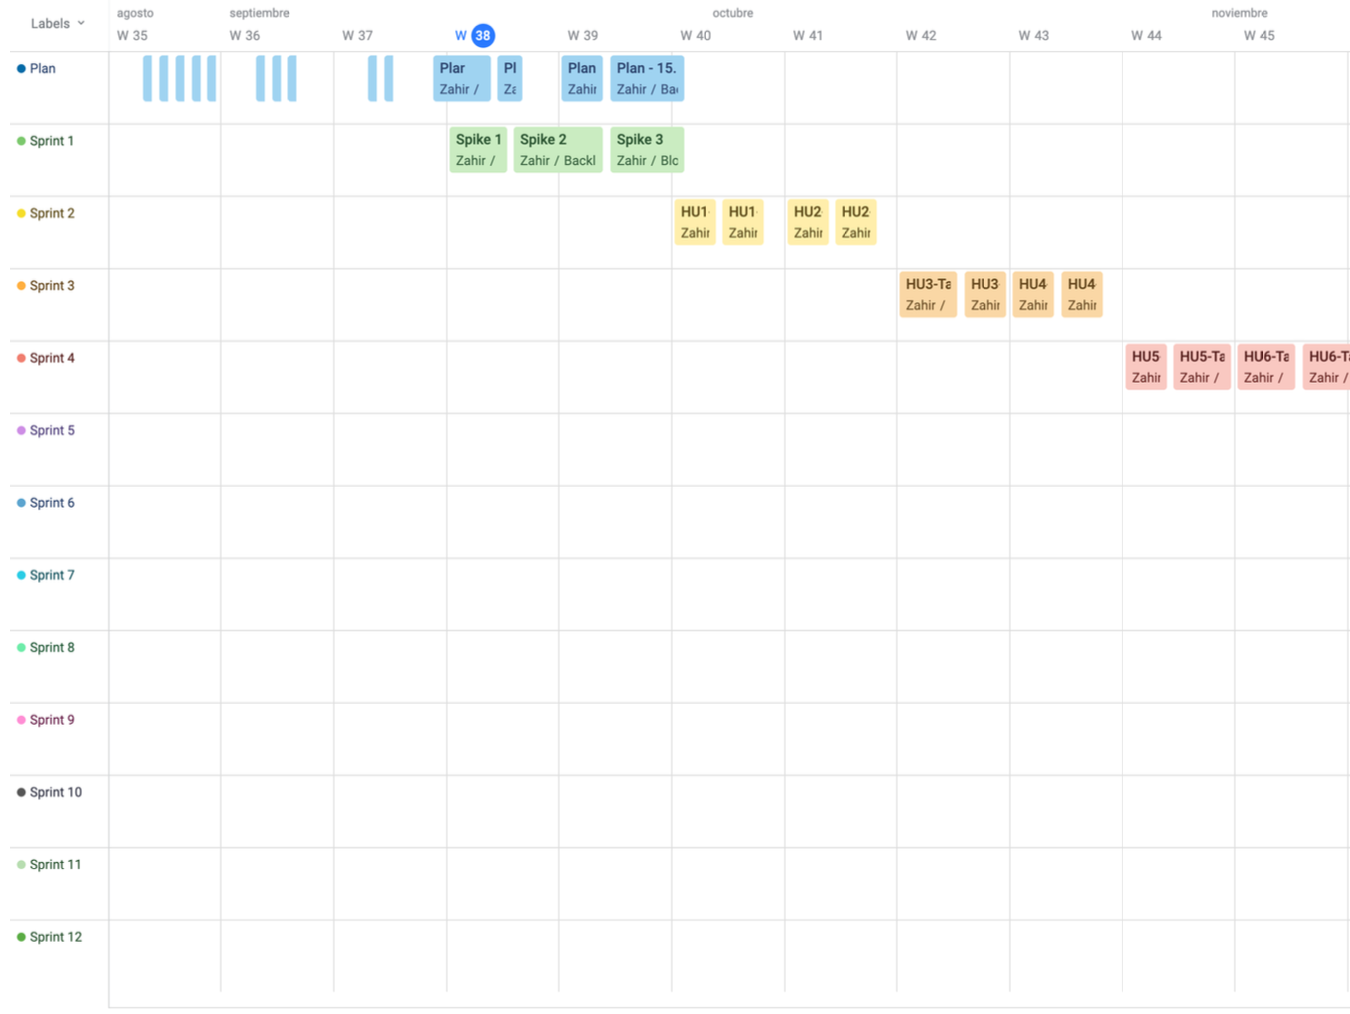
\includegraphics[height=6cm]{./Figuras/Gantt-1.png}
\end{minipage}%
%\hfill
\begin{minipage}{0.50\textwidth}
%    \centering
    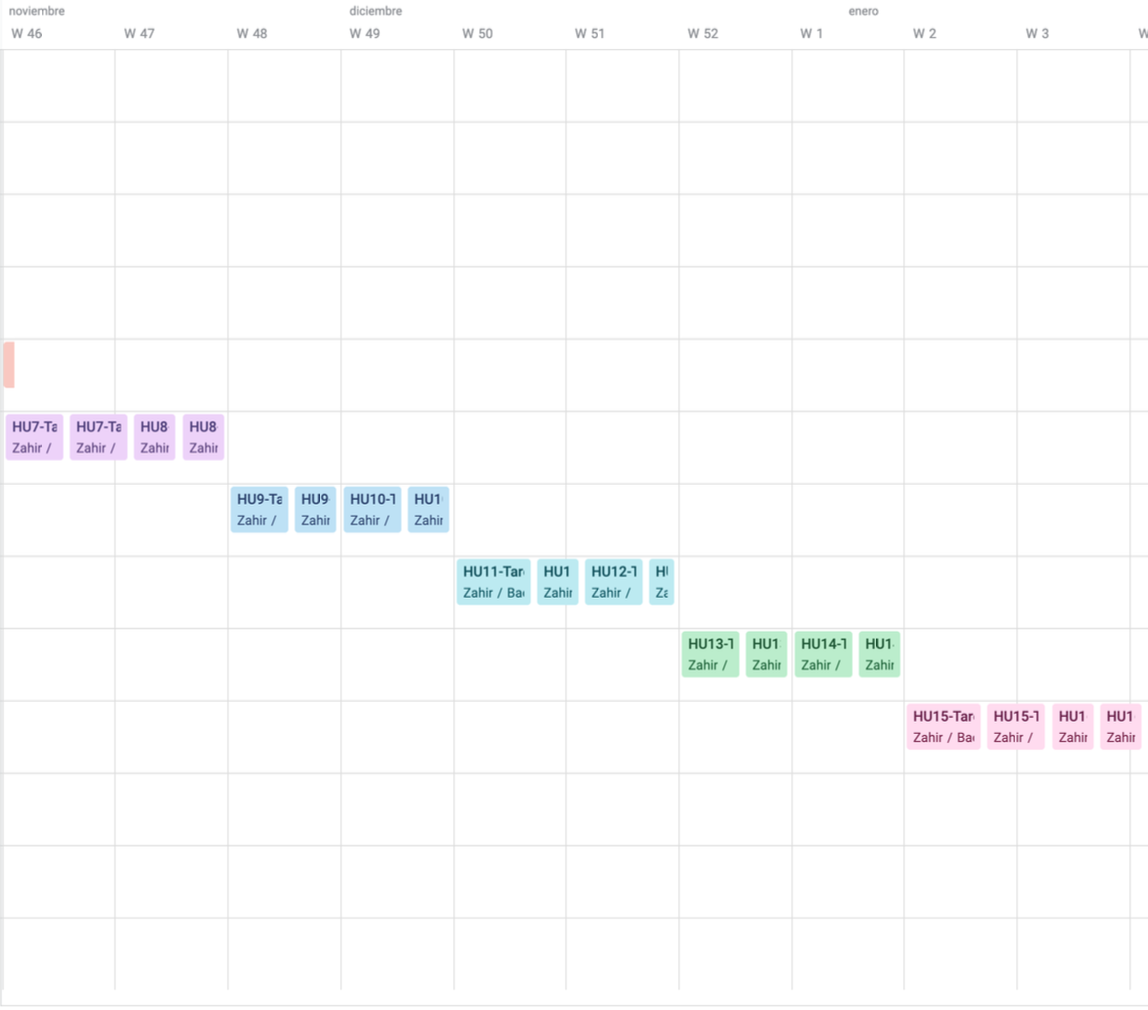
\includegraphics[height=6cm]{./Figuras/Gantt-2.png}
\end{minipage}%
\caption{Gantt: hasta el sprint 9.}

\vspace{0.5cm} % Space between rows

% Second row
\begin{minipage}{0.28\textwidth}
%    \centering
    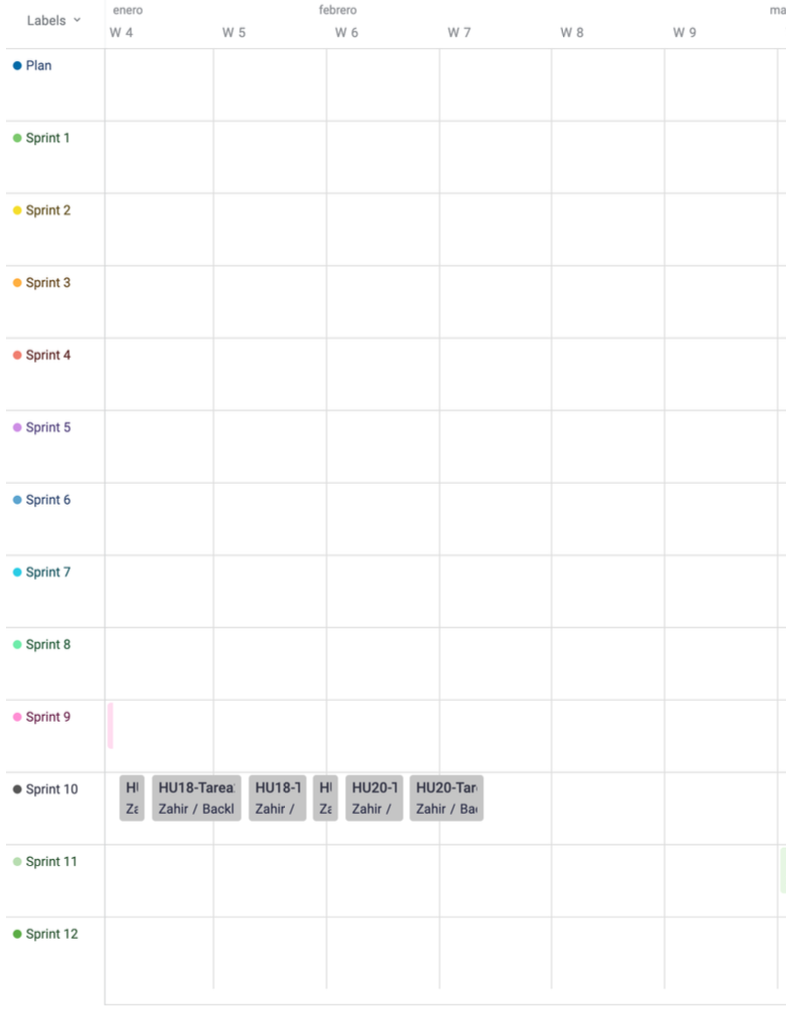
\includegraphics[height=6cm]{./Figuras/Gantt-3.png}
\end{minipage}%
%\hfill
\begin{minipage}{0.72\textwidth}
%    \centering
    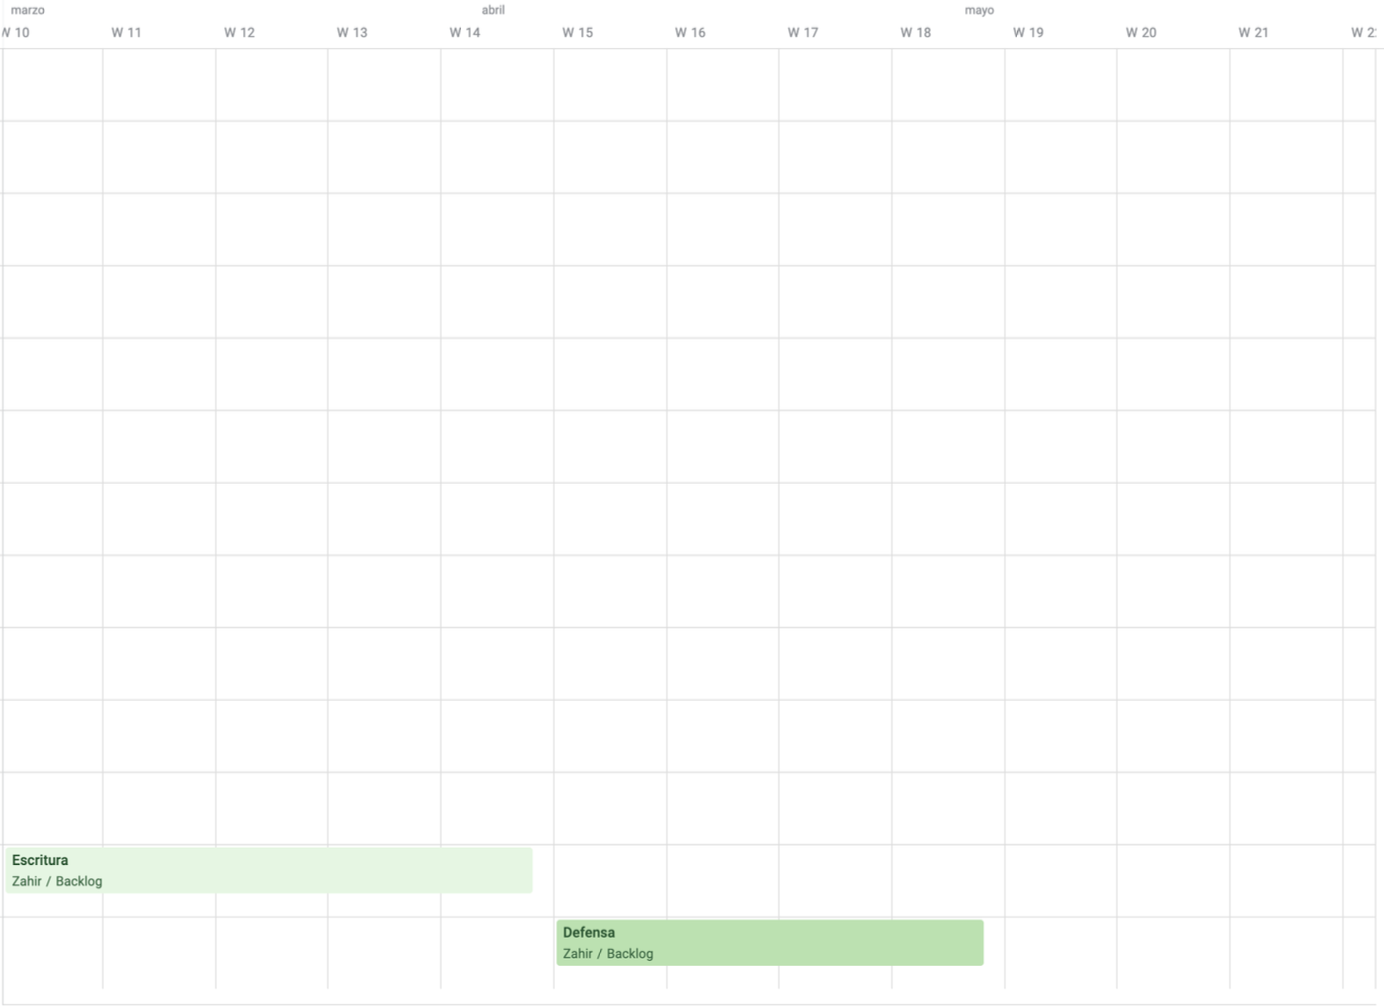
\includegraphics[height=6cm]{./Figuras/Gantt-4.png}
\end{minipage}%

\caption{Gantt sprints 10 al 12.}
\label{fig:diagBloques}
\end{flushleft}
\end{figure}

%\begin{figure}[htpb]
%\centering 
%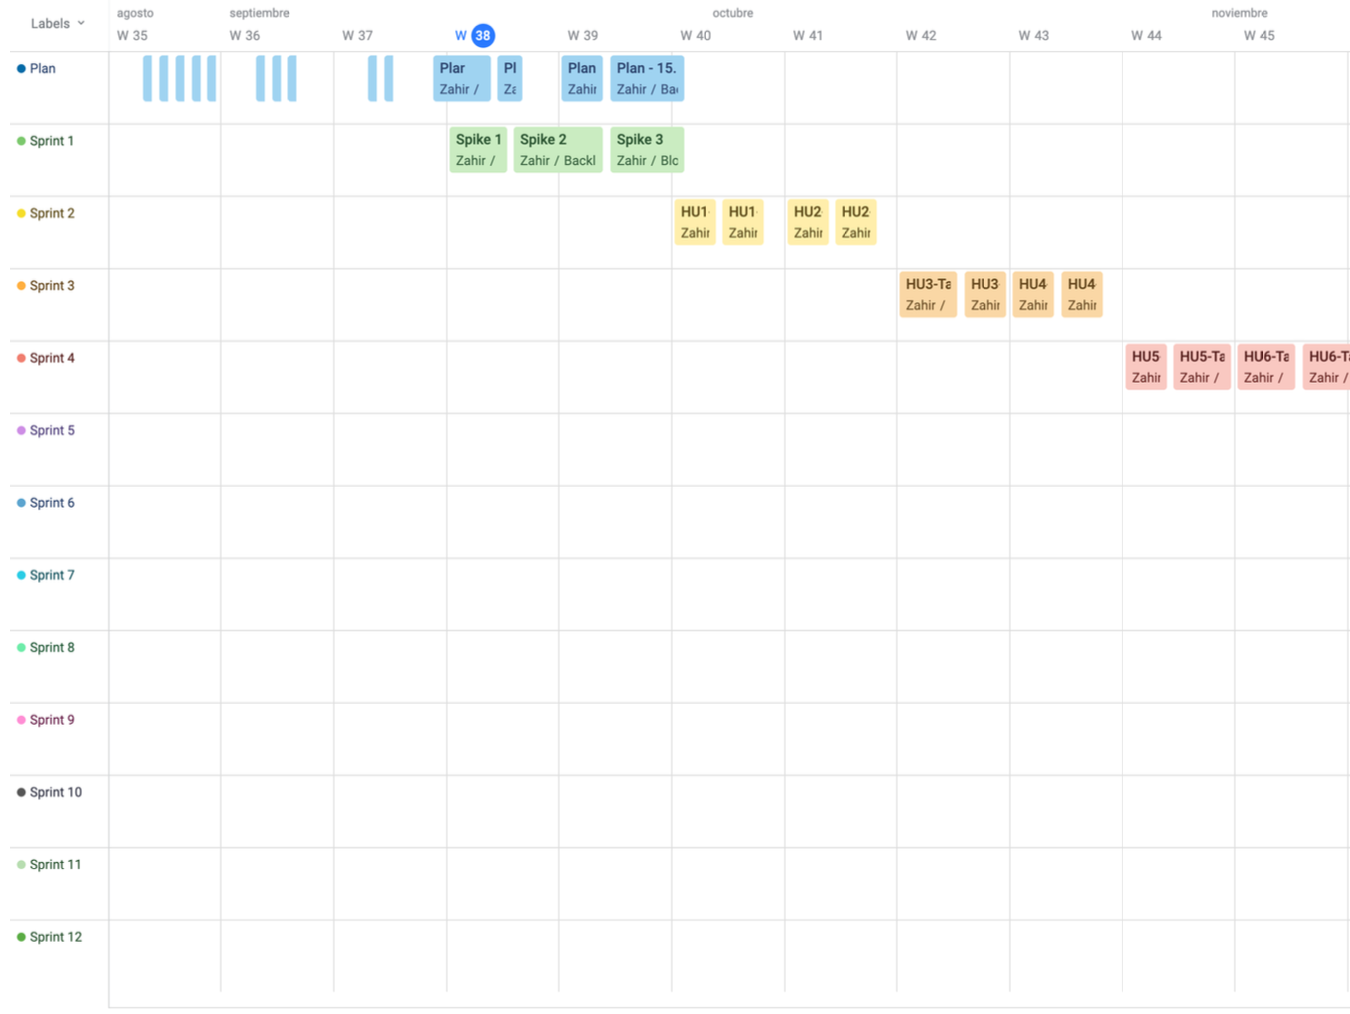
\includegraphics[width=.65\textwidth]{./Figuras/Gantt-1.png}
%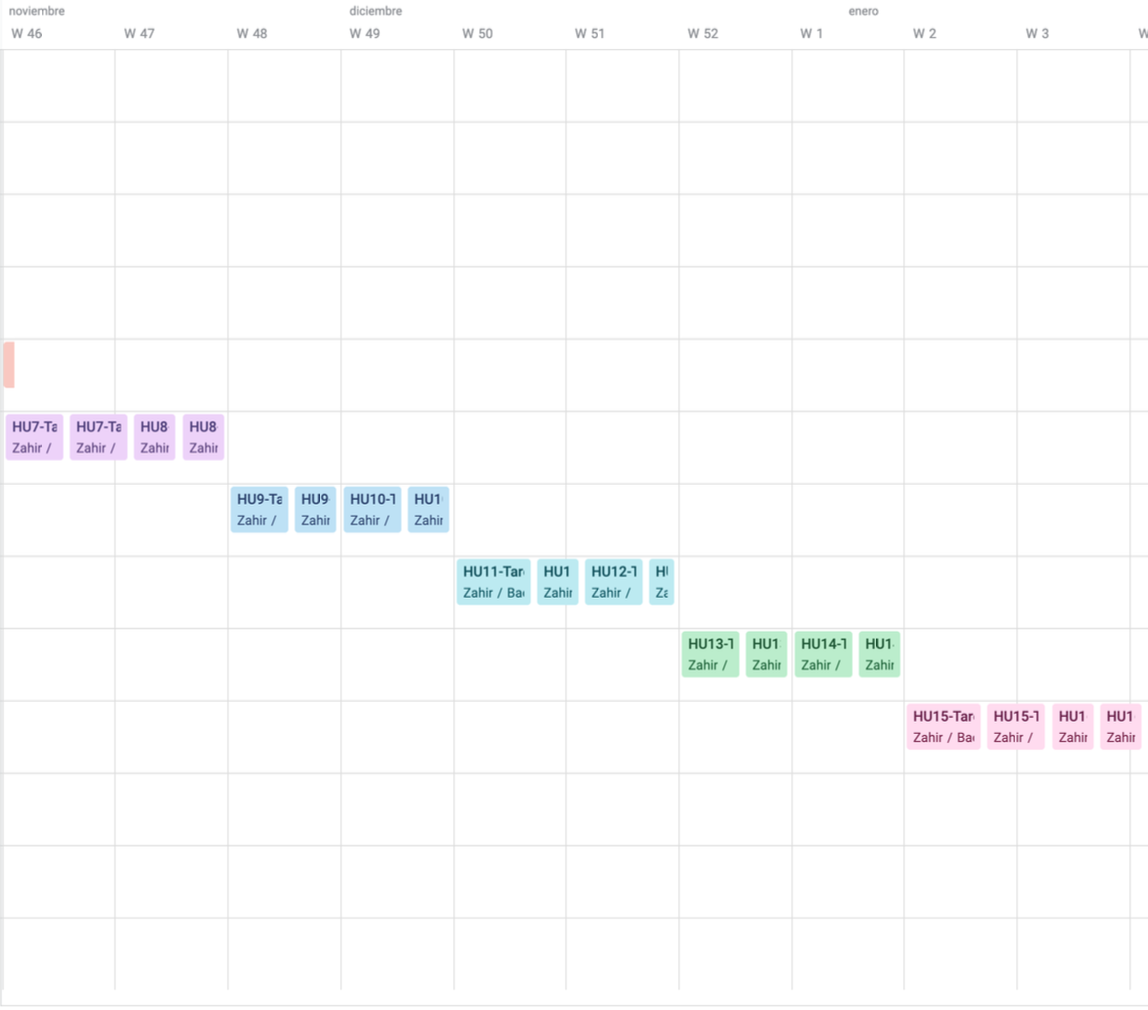
\includegraphics[width=.65\textwidth]{./Figuras/Gantt-2.png}
%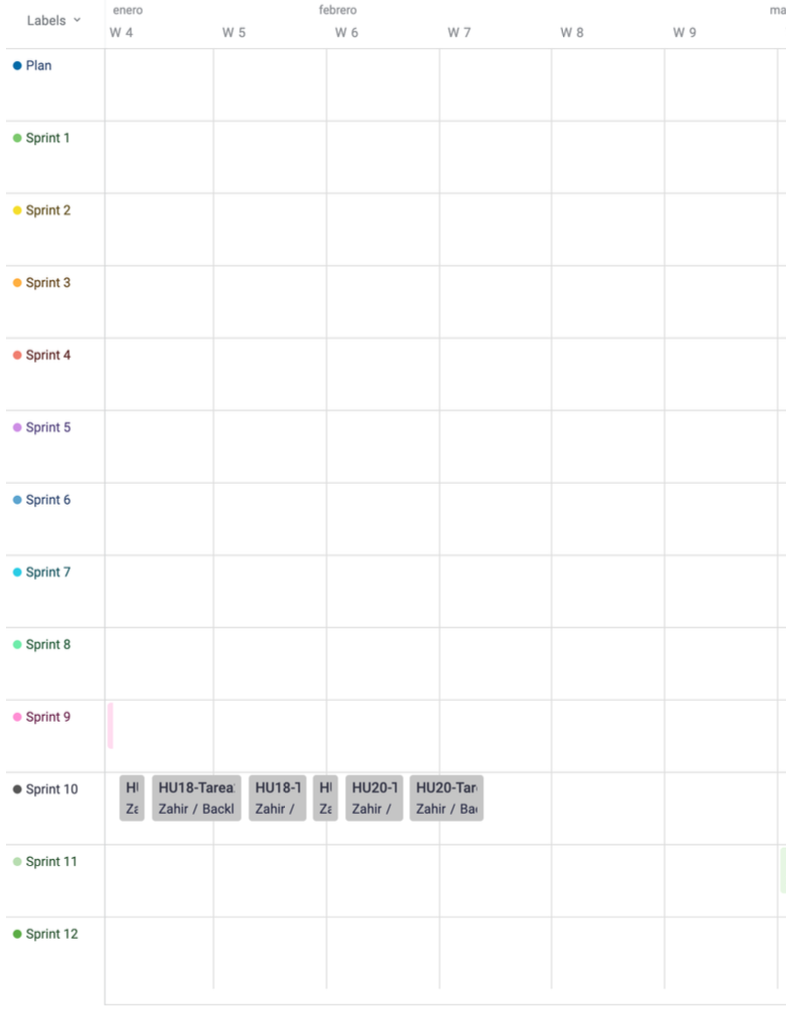
\includegraphics[width=.65\textwidth]{./Figuras/Gantt-3.png}
%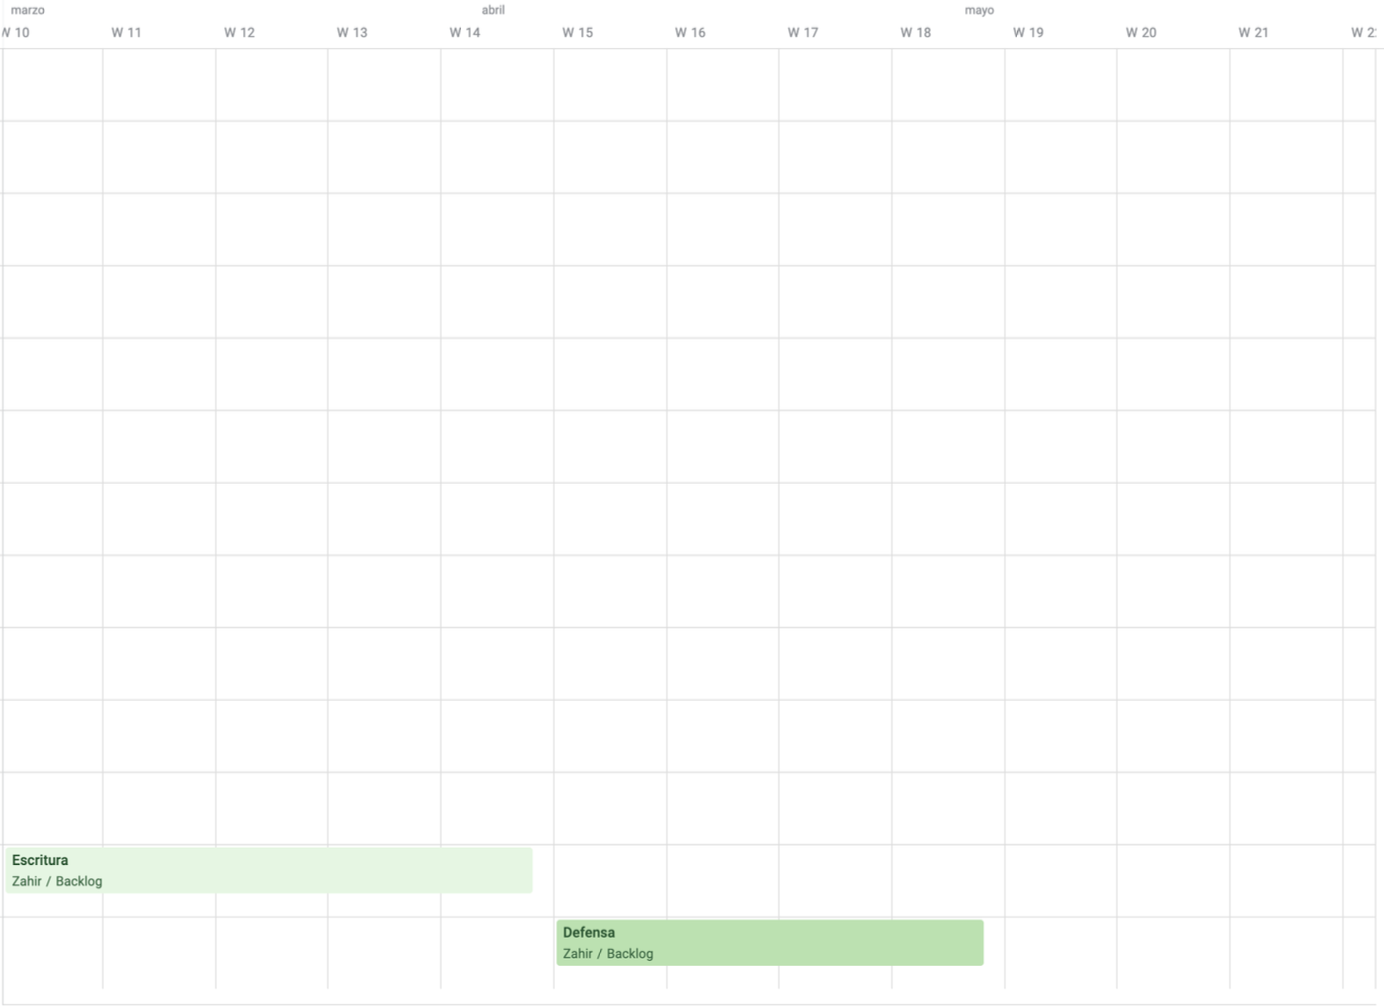
\includegraphics[width=.65\textwidth]{./Figuras/Gantt-4.png}
%\caption{Diagrama de Gantt.}
%\label{fig:diagBloques}
%\end{figure}

\vspace{25px}
%En la figura se puede observar un actor que provee los archivos de las canciones que son las entradas del sistema IA, donde se procesa cada canción para extraer sus características musicales. Las características son las salidas, y son almacenadas en una base de datos que alimenta el \textit{backend} de la aplicación. Ahora, en la figura 2, se muestra un diagrama de bloques más detallado del sistema IA. 

\newpage
\section{12. Normativa y cumplimiento de datos (gobernanza)}

En este proyecto no se analizan ni se almacenan datos personales de individuos, por lo que no resulta aplicable la normativa de protección de datos personales (como el Reglamento General de Protección de Datos --GDPR-- en la Unión Europea o la Ley 25.326 en Argentina). En consecuencia, no es necesario recabar consentimiento explícito de usuarios finales, dado que no se involucra información sensible ni identificable.

Los conjuntos de datos empleados provienen de dos tipos de fuentes:
\begin{itemize}
  \item \textit{Datasets} públicos: disponibles abiertamente para fines de investigación y desarrollo, sin restricciones contractuales adicionales.
  \item \textit{Dataset} privado del cliente: de propiedad exclusiva del cliente, autorizado para su uso en este proyecto académico. Para efectos de la evaluación del trabajo, se va a disponer de subconjuntos de datos o material de referencia compartible con el director y los jurados, preservando siempre los derechos de propiedad del cliente.
\end{itemize}

Es importante aclarar que los archivos de audio contenidos en los \textit{datasets}, tanto públicos como privados, son propiedad intelectual de sus respectivos compositores e intérpretes. El proyecto no transfiere ni modifica esos derechos, limitándose al uso autorizado de copias digitales para fines de análisis técnico y académico.

En términos de propiedad y derechos sobre los resultados del proyecto, estos corresponden de forma conjunta al cliente y al alumno, de acuerdo con los acuerdos establecidos. 

En conclusión, el proyecto cumple con la normativa vigente en materia de gobernanza de datos, respeta los derechos de propiedad intelectual de terceros y establece claramente las condiciones de uso de los \textit{datasets} empleados, garantizando la viabilidad legal y ética de la investigación.
%En esta sección se debe analizar si los datos utilizados en el proyecto están sujetos a normativas de protección de datos y privacidad, y en qué condiciones se pueden emplear.
%\textbf{Aspectos a considerar:}
%\begin{itemize}
%  \item Evaluar si los datos están regulados por normativas como GDPR, Ley 25.326 de Protección de Datos Personales en Argentina, HIPAA u otras según jurisdicción y temática.
%  \item Determinar si el uso de los datos requiere consentimiento explícito de los usuarios involucrados.
%  \item Indicar si existen restricciones legales, técnicas o contractuales sobre el uso, compartición o publicación de los datos.
%  \item Aclarar si los datos provienen de fuentes licenciadas, de acceso público o bajo algún tipo de autorización especial.
%  \item Analizar la viabilidad del proyecto desde el punto de vista legal y ético, considerando la gobernanza de los datos.
%\end{itemize}

%Este análisis es clave para garantizar el cumplimiento normativo y evitar conflictos legales durante el desarrollo y publicación del proyecto.En este proyecto no se analizan ni se almacenan datos personales de individuos, por lo que no resulta aplicable la normativa de protección de datos personales (como el Reglamento General de Protección de Datos --GDPR-- en la Unión Europea o la Ley 25.326 en Argentina). En consecuencia, no es necesario recabar consentimiento explícito de usuarios finales, dado que no se involucra información sensible ni identificable.

\section{13. Gestión de riesgos}
\label{sec:riesgos}

\begin{consigna}{red}
a) Identificación de los riesgos (al menos cinco) y estimación de sus consecuencias:
 
Riesgo 1: detallar el riesgo (riesgo es algo que si ocurre altera los planes previstos de forma negativa)
\begin{itemize}
	\item Severidad (S): mientras más severo, más alto es el número (usar números del 1 al 10).\\
	Justificar el motivo por el cual se asigna determinado número de severidad (S).
	\item Probabilidad de ocurrencia (O): mientras más probable, más alto es el número (usar del 1 al 10).\\
	Justificar el motivo por el cual se asigna determinado número de (O). 
\end{itemize}   

Riesgo 2:
\begin{itemize}
	\item Severidad (S): X.\\
	Justificación...
	\item Ocurrencia (O): Y.\\
	Justificación...
\end{itemize}

Riesgo 3:
\begin{itemize}
	\item Severidad (S):  X.\\
	Justificación...
	\item Ocurrencia (O): Y.\\
	Justificación...
\end{itemize}


b) Tabla de gestión de riesgos:      (El RPN se calcula como RPN=SxO)

\begin{table}[htpb]
\centering
\begin{tabularx}{\linewidth}{@{}|X|c|c|c|c|c|c|@{}}
\hline
\rowcolor[HTML]{C0C0C0} 
Riesgo & S & O & RPN & S* & O* & RPN* \\ \hline
       &   &   &     &    &    &      \\ \hline
       &   &   &     &    &    &      \\ \hline
       &   &   &     &    &    &      \\ \hline
       &   &   &     &    &    &      \\ \hline
       &   &   &     &    &    &      \\ \hline
\end{tabularx}%
\end{table}

Criterio adoptado: 

Se tomarán medidas de mitigación en los riesgos cuyos números de RPN sean mayores a...

Nota: los valores marcados con (*) en la tabla corresponden luego de haber aplicado la mitigación.

c) Plan de mitigación de los riesgos que originalmente excedían el RPN máximo establecido:
 
Riesgo 1: plan de mitigación (si por el RPN fuera necesario elaborar un plan de mitigación).
  Nueva asignación de S y O, con su respectiva justificación:
  \begin{itemize}
	\item Severidad (S*): mientras más severo, más alto es el número (usar números del 1 al 10).
          Justificar el motivo por el cual se asigna determinado número de severidad (S).
	\item Probabilidad de ocurrencia (O*): mientras más probable, más alto es el número (usar del 1 al 10).
          Justificar el motivo por el cual se asigna determinado número de (O).
	\end{itemize}

Riesgo 2: plan de mitigación (si por el RPN fuera necesario elaborar un plan de mitigación).
 
Riesgo 3: plan de mitigación (si por el RPN fuera necesario elaborar un plan de mitigación).

\end{consigna}

\section{14. Sprint Review}
\label{sec:sprint_review}

La revisión de sprint (\emph{Sprint Review}) es una práctica fundamental en metodologías ágiles. Consiste en revisar y evaluar lo que se ha completado al finalizar un sprint. En esta instancia, se presentan los avances y se verifica si las funcionalidades cumplen con los criterios de aceptación establecidos. También se identifican entregables parciales y se consideran ajustes si es necesario.

Aunque el proyecto aún se encuentre en etapa de planificación, esta sección permite proyectar cómo se evaluarán las funcionalidades más importantes del backlog. Esta mirada anticipada favorece la planificación enfocada en valor y permite reflexionar sobre posibles obstáculos.

\textbf{Objetivo:} anticipar cómo se evaluará el avance del proyecto a medida que se desarrollen las funcionalidades, utilizando como base al menos cuatro historias de usuario del \emph{Product Backlog}.


Seleccionar al menos 4 HU del Product Backlog. Para cada una, completar la siguiente tabla de revisión proyectada:

\textbf{Formato sugerido:}
\begin{table}[htpb]
\renewcommand{\arraystretch}{1.5}
\begin{tabular}{|>{\raggedright\arraybackslash}m{2.4cm}|
                >{\raggedright\arraybackslash}m{2.3cm}|
                >{\raggedright\arraybackslash}m{3cm}|
                >{\raggedright\arraybackslash}m{3cm}|
                >{\raggedright\arraybackslash}m{3cm}|}
\hline
\rowcolor[HTML]{CCCCCC}
\textbf{HU seleccionada} & \textbf{Tareas asociadas} & \textbf{Entregable esperado} & \textbf{¿Cómo sabrás que está cumplida?} & \textbf{Observaciones o riesgos} \\
\hline
                         & Tarea 1 &                             &                                           &                                     \\ \cline{2-2}
\multirow{-2}{=}{HU1}    & Tarea 2 & \multirow{-2}{=}{Módulo funcional} & \multirow{-2}{=}{Cumple criterios de aceptación definidos} & \multirow{-2}{=}{Falta validar con el tutor} \\
\hline
                         & Tarea 1 &                             &                                           &                                     \\ \cline{2-2}
\multirow{-2}{=}{HU3}    & Tarea 2 & \multirow{-2}{=}{Reporte generado} & \multirow{-2}{=}{Exportación disponible y clara} & \multirow{-2}{=}{Requiere datos reales} \\
\hline
                         & Tarea 1 &                             &                                           &                                     \\ \cline{2-2}
\multirow{-2}{=}{HU5}    & Tarea 2 & \multirow{-2}{=}{Panel de gestión} & \multirow{-2}{=}{Roles diferenciados operativos} & \multirow{-2}{=}{Riesgo en integración} \\
\hline
                         & Tarea 1 &                             &                                           &                                     \\ \cline{2-2}
\multirow{-2}{=}{HU7}    & Tarea 2 & \multirow{-2}{=}{Informe trimestral} & \multirow{-2}{=}{PDF con gráficos y evolución} & \multirow{-2}{=}{Puede faltar tiempo para ajustes} \\
\hline
\end{tabular}
\end{table}

\section{15. Sprint Retrospective}    
\label{sec:sprint_retro}

La retrospectiva de sprint es una práctica orientada a la mejora continua. Al finalizar un sprint, el equipo (o el alumno, si trabaja de forma individual) reflexiona sobre lo que funcionó bien, lo que puede mejorarse y qué acciones concretas pueden implementarse para trabajar mejor en el futuro.

Durante la cursada se propuso el uso de la \textbf{Estrella de la Retrospectiva}, que organiza la reflexión en torno a cinco ejes:

\begin{itemize}
\item  ¿Qué hacer más?
\item  ¿Qué hacer menos?
\item  ¿Qué mantener?
\item  ¿Qué empezar a hacer?
\item  ¿Qué dejar de hacer?
\end{itemize}

Aun en una etapa temprana, esta herramienta permite que el alumno planifique su forma de trabajar, identifique anticipadamente posibles dificultades y diseñe estrategias de organización personal.

\textbf{Objetivo:} reflexionar sobre las condiciones iniciales del proyecto, identificando fortalezas, posibles dificultades y estrategias de mejora, incluso antes del inicio del desarrollo.


Completar la siguiente tabla tomando como referencia los cinco ejes de la Estrella de la Retrospectiva (\emph{Starfish} o estrella de mar). Esta instancia te ayudará a definir buenas prácticas desde el inicio y prepararte para enfrentar el trabajo de forma organizada y flexible. Se deberá completar la tabla al menos para 3 sprints técnicos y 1 no técnico.

\textbf{Formato sugerido:}

\begin{table}[htpb]
\renewcommand{\arraystretch}{1.4}
\begin{tabular}{|>{\raggedright\arraybackslash}p{1.8cm}|
                >{\raggedright\arraybackslash}p{2.3cm}|
                >{\raggedright\arraybackslash}p{2.3cm}|
                >{\raggedright\arraybackslash}p{2.3cm}|
                >{\raggedright\arraybackslash}p{2.3cm}|
                >{\raggedright\arraybackslash}p{2.3cm}|}
\hline
\rowcolor[HTML]{CCCCCC} 
\textbf{Sprint tipo y N°} & \textbf{¿Qué hacer más?} & \textbf{¿Qué hacer menos?} & \textbf{¿Qué mantener?} & \textbf{¿Qué empezar a hacer?} & \textbf{¿Qué dejar de hacer?} \\
\hline
Sprint técnico - 1 & Validaciones continuas con el alumno & Cambios sin versión registrada & Pruebas con datos simulados & Documentar cambios propuestos & Ajustes sin análisis de impacto \\
\hline
Sprint técnico - 2 & Verificar configuraciones en múltiples escenarios & Modificar parámetros sin guardar historial & Perfiles reutilizables & Usar logs para configuración & Repetir pruebas manuales innecesarias \\
\hline
Sprint técnico - 8 & Comparar correlaciones con casos previos & Cambiar parámetros sin justificar & Revisión cruzada de métricas & Anotar configuraciones usadas & Trabajar sin respaldo de datos \\
\hline
Sprint no técnico - 12 (por ej.: ``Defensa'') & Ensayos orales con feedback & Cambiar contenidos en la memoria & Material visual claro & Dividir la presentación por bloques & Agregar gráficos difíciles de explicar \\
\hline
\end{tabular}
\end{table}




\end{document}